\let\negmedspace\undefined
\let\negthickspace\undefined
\documentclass[journal]{IEEEtran}
\usepackage[a5paper, margin=10mm, onecolumn]{geometry}
%\usepackage{lmodern} % Ensure lmodern is loaded for pdflatex
\usepackage{tfrupee} % Include tfrupee package

\setlength{\headheight}{1cm} % Set the height of the header box
\setlength{\headsep}{0mm}     % Set the distance between the header box and the top of the text

\usepackage{gvv-book}
\usepackage{gvv}
\usepackage{cite}
\usepackage{amsmath,amssymb,amsfonts,amsthm}
\usepackage{algorithmic}
\usepackage{graphicx}
\usepackage{textcomp}
\usepackage{xcolor}
\usepackage{txfonts}
\usepackage{listings}
\usepackage{enumitem}
\usepackage{mathtools}
\usepackage{gensymb}
\usepackage{comment}
\usepackage[breaklinks=true]{hyperref}
\usepackage{tkz-euclide} 
\usepackage{listings}
% \usepackage{gvv}                                        
\def\inputGnumericTable{}                                 
\usepackage[latin1]{inputenc}                                
\usepackage{color}                                            
\usepackage{array}                                            
\usepackage{longtable}                                       
\usepackage{calc}                                             
\usepackage{multirow}                                         
\usepackage{hhline}                                           
\usepackage{ifthen}                                           
\usepackage{lscape}
\begin{document}

\bibliographystyle{IEEEtran}
\vspace{3cm}

\title{9.4.12}
\author{EE24BTECH11012 - Bhavanisankar G S}
% \maketitle
% \newpage
% \bigskip
{\let\newpage\relax\maketitle}

\renewcommand{\thefigure}{\theenumi}
\renewcommand{\thetable}{\theenumi}
\setlength{\intextsep}{10pt} % Space between text and floats


\numberwithin{equation}{enumi}
\numberwithin{figure}{enumi}
\renewcommand{\thetable}{\theenumi}

\textbf{QUESTION} : \\
For the differential equation, $x (x^2 - 1) \frac{dy}{dx} = 1$, find the particular solution given that $y(2) = 0$. \\
\textbf{SOLUTION} : \\
\textbf{Theoritical} : \\
Consider the given equation, 
\begin{align}
	x \brak{x^2 - 1} \frac{dy}{dx} &= 1 \\
	\frac{dy}{dx} &= \frac{1}{x \brak{x^2 -1}} \label{eq:de} \\
	y(2) &= 0 \label{eq:ic}
\end{align}
By the method of \textbf{Partial fractions}, we have \\
\begin{align}
	\frac{dy}{dx} &= \frac{1}{2} \brak{\frac{1}{x-1}} + \frac{1}{2} \brak{\frac{1}{x+1}} - \frac{1}{x} \label{eq:int}
\end{align}
Integrating \eqref{eq:int} on both the sides, we have
\begin{align}
	\int dy &= \int \brak{\frac{1}{2} \brak{\frac{1}{x-1}} + \frac{1}{2} \brak{\frac{1}{x+1}} - \frac{1}{x}} dx \\
	y &= \frac{1}{2} \log{\abs{x-1}} + \frac{1}{2} \log{\abs{x+1}} - \log{\abs{x}} + \log{c} \\
	y &= \log \brak{\frac{c\sqrt{x^2 - 1}}{x}}
\end{align}
Substituting the initial conditions in \eqref{eq:ic}, we have
\begin{align}
	0 &= \log \brak{\frac{c\sqrt{2^2 - 1}}{2}} \\
	c &= \frac{2}{\sqrt{3}}
\end{align}
Hence, the required particular solution becomes
\begin{align}
	y &= \log \brak{\frac{2\sqrt{x^2 - 1}}{\sqrt{3} x}} 
\end{align}
\\ \\
\textbf{Simulation} : 
\begin{enumerate}
\item For a general interval, say $\sbrak{a,b}$, split up the intervals into $n$ parts such that
\begin{align}
	h &= \frac{b-a}{n} \label{eq:split}
\end{align}
\item Consider the points 
\begin{align}
	x_{0} &= a \\
	x_{n} &= b \\
	x_{i+1} &= x_{i} + h
\end{align}
\item \textbf{Trapezoid rule} : \\
Summing the areas of the trapezoids formed, we have
\begin{align}
	f(x) &= \frac{1}{x \brak{x^2 - 1}} \\
	A &\approx \frac{h}{2} \brak{(f(x_{0}) + f(x_{1})) + (f(x_{1}) + f(x_{2})) + \dots + (f(x_{n-1}) + f(x_{n}))} \\
	A &\approx \frac{h}{2} \brak{f(x_{0}) + 2 \sum_{i=1}^{n-1} f(x_{i}) + f(x_{n}) } \label{eq:dif}
\end{align}
\item To set up the difference equation, we integrate the equation \eqref{eq:de} from $n-1$ to $n$.
	\begin{align}
		a &= n-1 \\
		b &= n
	\end{align}
		On further simplifying the equation \eqref{eq:dif}, we have
		\begin{align}
			y_{n+1} - y_{n} &= \brak{x_{n+1} - x_{n}} \brak{\frac{f(x_{n})}{2} + \frac{f(x_{n+1})}{2}} \\
			y_{n+1} &= y_{n} + \brak{x_{n+1} - x_{n}} \brak{\frac{f(x_{n})}{2} + \frac{f(x_{n+1})}{2}} \\
			y_{n+1} &= y_{n} + \frac{\brak{x_{n+1} - x_{n}}}{2} \brak{\frac{1}{x_{n}(x_{n}^2 - 1)} + \frac{1}{x_{n+1}(x_{n+1}^2 - 1)}} \label{eq:difeq1} 
		\end{align}
		which is the required difference equation.
	\item Taking $x_0 = 2$ and $y_0 = 0$ and iterating \eqref{eq:difeq1}, we can obtain the other points.\\

\textbf{Another approach} : \\
Consider \eqref{eq:de}. Let the Laplace transform of RHS be $X(s)$. Then, 
\begin{align}
	g(t) &= \frac{1}{t(t^2 - 1)} \\
	\frac{dy}{dt} &= g(t) \label{eq:1}
\end{align}
Applying Laplace transform on both the sides of \eqref{eq:1} , we have 
\begin{align}
	s Y(s) &= X(s) 
\end{align}
The transfer function, $H(s)$ can then be defined as
\begin{align}
	H(s) &= \frac{Y(s)}{X(s)} \\
	H(s) &= \frac{1}{s} \label{eq:bil}
\end{align}
Applying \textbf{Bi-linear transform} on both sides of \eqref{eq:bil}, i.e., converting $s$-domain into $z$-domain, we have
\begin{align}
	s &= \frac{2}{h} \brak{\frac{1 - z^{-1}}{1 + z^{-1}}} \\
	H(z) &= \frac{h}{2} \brak{\frac{1 + z^{-1}}{1 - z^{-1}}} \\
	Y(z) &= \frac{h}{2} \brak{\frac{1 + z^{-1}}{1 - z^{-1}}} X(z) \\
	\brak{1 - z^{-1}} Y(z) &= \frac{h}{2} \brak{1 + z^{-1}} X(z) \label{eq:iz} 
\end{align}
Taking \textbf{Inverse z-transform} on both the sides of \eqref{eq:iz} , we have
\begin{align}
	y_{n} - y_{n-1} &= \frac{h}{2} \brak{g(x_{n}) + g(x_{n-1})} \\
	y_{n} &= y_{n-1} + \frac{h}{2} \brak{g(x_{n}) + g(x_{n-1})} \label{eq:difeq2}
\end{align}
which is the required difference equation. \\
It can be seen that \eqref{eq:difeq1} and \eqref{eq:difeq2} are essentially the same. \\
\textbf{Using RK method} : \\
By the method of \textbf{Finite differences}, we have \\
\begin{align}
	y(x + h) &= y(x) + y^{\prime}(x,y) h \label{eq:fd}
\end{align}
According to the RK method, \eqref{eq:fd} can be written as
\begin{align}
	y^{\prime} (x,y) &= \frac{1}{x \brak{x^2 - 1}} \\
	y(x_0 + h) &= y(x_0) + \frac{1}{6} \brak{k_1 + 2k_2 + 2k_3 + k_4} \label{eq:rk}
\end{align}
where, 
\begin{align}
	k_1 &= h y^{\prime} \brak{x_0, y_0} \\
	k_2 &= h y^{\prime} \brak{x_0 + \frac{h}{2}, y_0 + \frac{k_1}{2}} \\
	k_3 &= h y^{\prime} \brak{x_0 + \frac{h}{2}, y_0 + \frac{k_2}{2}} \\
	k_4 &= h y^{\prime} \brak{x_0 + h, y_0 + k_3}
\end{align}
Iterating \eqref{eq:rk}, a graph can be plotted. \\
Theoritical and simulation graphs of the methods described above are plotted below.

		\begin{figure}[h]
			\centering
			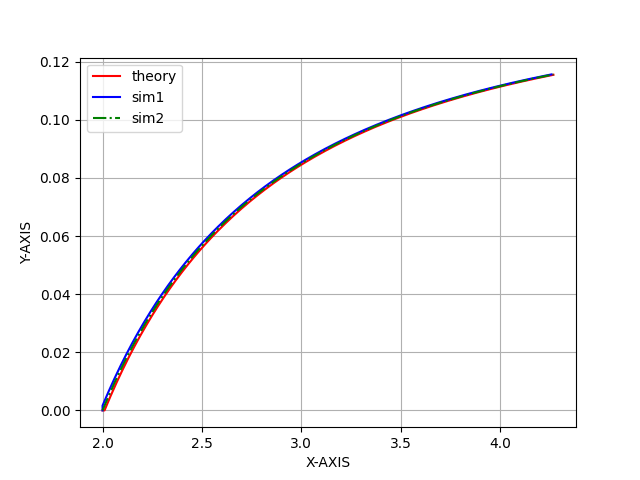
\includegraphics[width=\columnwidth]{figs/fig.png}
			\caption{Plot of the given question.}
			\label{fig:Plot1} 
		\end{figure}
\end{enumerate}
\end{document}
